%% Template for a preprint Letter or Article for submission
%% to the journal Nature.
%% Written by Peter Czoschke, 26 February 2004
%%

\documentclass{nature}

\usepackage{amsmath}
\usepackage{amssymb}
\usepackage{bm}
\usepackage{graphicx}

\def\aap{A\&A}
\def\aaps{A\&AS}
\def\aapr{A\&ARv}
\def\aarv{A\&ARv}
\def\aj{AJ}
\def\ao{ApOpt}
\def\apj{ApJ}
\def\apjl{ApJL}
\def\apjs{ApJS}
\def\apss{Ap\&SS}
\def\araa{ARA\&A}
\def\aspc{ASPC}
\def\bjp{Braz.\ J.\ Phys.}
\def\casp{Comm.\ Astrophys.\ Space Phys.}
\def\helv{Helv.\ Phys.\ Acta}
\def\jcap{JCAP}
\def\mnras{MNRAS}
\def\nat{Nature}
\def\nature{Nature}
\def\njph{New.\ J.\ Phys.}
\def\obs{Observatory}
\def\pasa{PASA}
\def\pasp{PASP}
\def\physrep{Phys.\ Rep.}
\def\pnas{PNAS}
\def\prd{PhRvD}
\def\procspie{SPIE}
\def\ssr{Space Sci.\ Rev.}


%% make sure you have the nature.cls and naturemag.bst files where
%% LaTeX can find them

\bibliographystyle{naturemag}


\title{Weak lensing masses of Ultra Diffuse Galaxies in nearby galaxy clusters}

%% Notice placement of commas and superscripts and use of &
%% in the author list

\author{Crist\'obal~Sif\'on$^{1,2}$, Remco~F.~J.~van~der~Burg$^3$, Adam~Muzzin$^4$, Henk~Hoekstra$^2$ \& Ricardo~Herbonnet$^2$}


\begin{document}

\maketitle

\begin{affiliations}
 \item Department of Astrophysical Sciences, Peyton Hall, Princeton University, Princeton, NJ 08544, USA
 \item Leiden Observatory, Leiden University, PO Box 9513, NL-2300 RA Leiden, The Netherlands
 \item Laboratoire AIM, IRFU/Service d’Astrophysique - CEA/DSM - CNRS - Universit\'e Paris Diderot, B\^{a}t. 709, CEA-Saclay, 91191 Gif-sur-Yvette Cedex, France
 \item York University
\end{affiliations}

\begin{abstract}
    The recent discovery of large populations of ultra diffuse galaxies (UDGs) in nearby galaxy clusters\cite{koda15,vandokkum15,vdburg16} has opened a new window into the process of galaxy formation and evolution. These galaxies have as much stellar matter as dwarf galaxies but appear as large in size as the Milky Way
\end{abstract}

Then the body of the main text appears after the intro paragraph.
Figure environments can be left in place in the document.
\verb|\includegraphics| commands are ignored since Nature wants
the figures sent as separate files and the captions are
automatically moved to the end of the document (they are printed
out with the \verb|\end{document}| command. However, tables must
be manually moved to the end of the document, after the addendum.

\begin{figure}
 \centerline{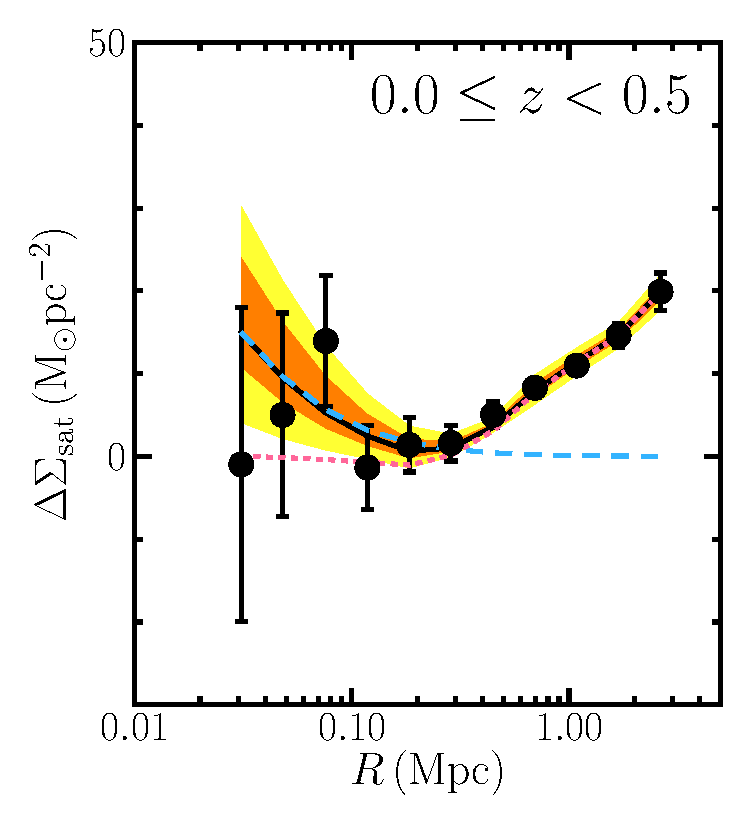
\includegraphics[width=3in]{test.pdf}}
\caption{Each figure legend should begin with a brief title for
the whole figure and continue with a short description of each
panel and the symbols used. For contributions with methods
sections, legends should not contain any details of methods, or
exceed 100 words (fewer than 500 words in total for the whole
paper). In contributions without methods sections, legends should
be fewer than 300 words (800 words or fewer in total for the whole
paper).}
\end{figure}


%% Put the bibliography here, most people will use BiBTeX in
%% which case the environment below should be replaced with
%% the \bibliography{} command.

% \begin{thebibliography}{1}
% \bibitem{dummy} Articles are restricted to 50 references, Letters
% to 30.
% \bibitem{dummyb} No compound references -- only one source per
% reference.
% \end{thebibliography}
\bibliography{bibliography}


%% Here is the endmatter stuff: Supplementary Info, etc.
%% Use \item's to separate, default label is "Acknowledgements"

% \begin{addendum}
%  \item Put acknowledgements here.
%  \item[Competing Interests] The authors declare that they have no
% competing financial interests.
%  \item[Correspondence] Correspondence and requests for materials
% should be addressed to A.B.C.~(email: myaddress@nowhere.edu).
% \end{addendum}

%%
%% TABLES
%%
%% If there are any tables, put them here.
%%

\end{document}
